
\begin{table*}[t]\centering\small
\begin{tabular}{lrrrrr}
\toprule
Model & NFE/frame & KTH pooled & KTH member & CLEVRER pooled & CLEVRER member \\
\midrule
SI & 16 & 1781.7 & 1812.6 $\pm$ 16.3 & 436.1 & 485.3 $\pm$ 16.2 \\
SI & 64 & 773.5 & 823.0 $\pm$ 20.7 & 222.3 & 268.9 $\pm$ 10.7 \\
FM & 16 & 726.8 & 766.9 $\pm$ 17.2 & 323.0 & 361.8 $\pm$ 19.1 \\
FM & 64 & 783.1 & 831.5 $\pm$ 21.7 & 330.0 & 372.1 $\pm$ 19.8 \\
It\^o map & 1 & 1271.3 & 1302.2 $\pm$ 18.8 & 1080.0 & 1117.4 $\pm$ 18.9 \\
It\^o map & 8 & 888.2 & 926.5 $\pm$ 21.1 & 317.3 & 360.5 $\pm$ 6.0 \\
Flow map & 1 & 857.2 & 895.1 $\pm$ 18.1 & 402.2 & 442.7 $\pm$ 5.4 \\
Flow map & 8 & 706.6 & 748.0 $\pm$ 19.0 & 320.4 & 359.9 $\pm$ 15.3 \\
Persistence & 0 & 816.1 & 815.8 $\pm$ 0.0 & 1072.2 & 1071.5 $\pm$ 0.0 \\
\bottomrule
\end{tabular}

\caption{Pixel-video FVD (lower is better). Pooled FVD compares 128 real and 512 generated clips. Member FVD reports mean $\pm$ completion SD of four separate 128-versus-128 comparisons, not confidence intervals. Cases are shared; each model uses one checkpoint at all its budgets. NFE is per generated frame and member; persistence uses none. Other metrics are in Appendix~\ref{app:video-results}.}\label{tab:video-main-fvd}
\end{table*}
\begin{figure*}[t]\centering
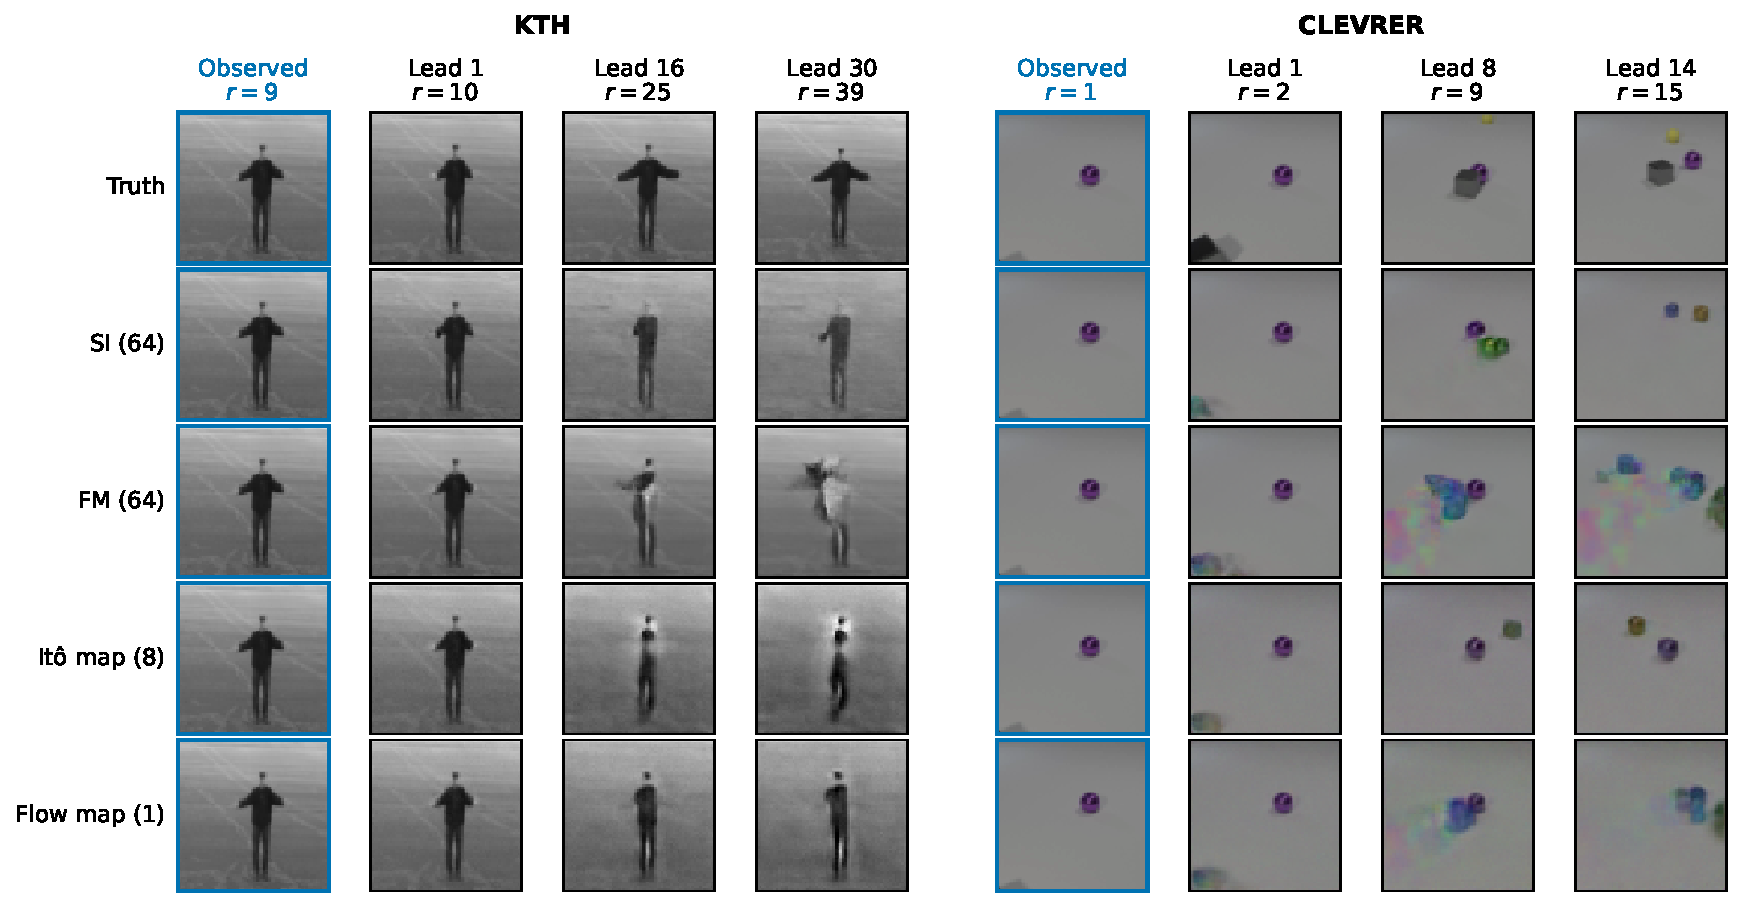
\includegraphics[width=\textwidth]{figures/video_results/main_forecast_sequences.pdf}
\caption{Matched observed and predicted frame sequences for both datasets. Rows show truth and one sampled completion from each model, never an ensemble average. The blue-bordered column repeats the last observed frame; remaining columns are forecasts. $r$ is the zero-based retained-frame index within the clip: KTH retains every frame; CLEVRER raw-frame index is $5r$. Cases are the first frozen selections, member zero, at prespecified budgets (parentheses). Display clipping does not alter feedback. The other observed history frames condition each model but are omitted for space.}\label{fig:video-main-sequences}
\end{figure*}
